In diesem Kapitel werden Grundlagen besprochen die eine Relevanz für diese Arbeit haben. Die angesprochenen Bereiche können nur oberflächlich einen kleinen Einstieg in die jeweiligen Teilgebiete geben.\vspace{0.2cm}

Die Forschungsbereiche der großen Sprachmodelle, kurz \acrshort{LLM} [eng. Large Language Model], ist ein Teilgebiet von Deep Learning und der Forschung von der Verarbeitung natürlicher Sprache, kurz \acrshort{NLP} [eng. Natural Language Processing]. Die Grafik \ref{img:classification_of_terms} zeigt die Einordnung der Bereiche.

\begin{figure}[!ht]
	\includegraphics[width=0.8\textwidth]{content/chapter_basics/images/einordnung_bezeichnungen.eps}
	\centering
	\caption{LLMs im Kontext der Forschungsbereiche von KI}
	\label{img:classification_of_terms}
\end{figure}


\section{Künstliche Intelligenz}
Die künstliche Intelligenz hat bereits in viele Unternehmensprozesse Einzug gehalten. Besonders die generative KI, mit ihren großen Sprachmodellen wird in den nächsten Jahren immer weiter in die Unternehmensbereiche vorstoßen und viele Aufgaben übernehmen. Entscheider und Führungspersonal versprechen sich von der Technologie nicht nur effizientere Prozesse, sondern auch Kosteneinsparungen.\vspace{0.2cm}

Eine explizite Definition für \textit{künstliche Intelligenz} ist zurzeit noch nicht einheitlich erfolgt. Geschuldet ist diese Tatsache, dass der Begriff \textit{Intelligenz} nicht eindeutig definiert ist. Somit finden sich viele Versuche eine Definition für künstliche Intelligenz herzuleiten. In dieser Arbeit wird als Definition für die Künstliche Intelligenz, die aus \cite[6 ff.]{definition_ki2019} verwendet.

\epigraph[
	author={Bitkom e.V.},
	text indent=0.5cm,
	after skip=-1.0cm
	]{
	Systeme der künstlichen Intelligenz (KI-Systeme) sind vom Menschen entwickelte Softwaresysteme (und gegebenenfalls auch Hardwaresysteme), die in Bezug auf ein komplexes Ziel auf physischer oder digitaler Ebene handeln, indem sie ihre Umgebung durch Datenerfassung wahrnehmen, die gesammelten strukturierten oder unstrukturierten Daten interpretieren, Schlussfolgerungen daraus ziehen oder die aus diesen Daten abgeleiteten Informationen verarbeiten, und über das bestmögliche Handeln zur Erreichung des vorgegebenen Ziels entscheiden. KI-Systeme können entweder symbolische Regeln verwenden oder ein numerisches Modell erlernen, und sind auch in der Lage, die Auswirkungen ihrer früheren Handlungen auf die Umgebung zu analysieren und ihr Verhalten entsprechend anzupassen.
}

%(\href{https://www.bitkom.org/sites/main/files/file/import/171012-KI-Gipfelpapier-online.pdf}{Wirtschaftliche Bedeutung ...}, 26 ff.).

%Die folgenden Kapitel werden auf die Teilbereiche der künstlichen Intelligenz eingehen, welche für die Entwicklung der großen Sprachmodelle essenziell sind.
Aus dem Forschungsgebiet der künstlichen Intelligenz ist für die großen Sprachmodelle der Bereich des \glqq Deep Learning\grqq \ besonders interessant. Hier findet die Überschneidung mit dem Bereich der NLP statt, welche massiv dazu betrug, dass die großen Sprachmodelle diesen Erfolg erfahren.

\subsection{Maschinelles Lernen}
Als Teilgebiet der künstlichen Intelligenz befasst es sich mit dem Problem wie Maschinen Lernen und Denken können. Wobei hier nicht von selbstständigem Lernen und Denken gesprochen werden kann, sondern lediglich von Imitieren dieser Prozesse. Aber \acrshort{ML} ist sehr wohl in der Lage aus großen Datenmengen komplexe Muster und Funktionen zu erkennen. Für das maschinelle Lernen gibt es mehrere Formen von Lernparadigmen.\vspace{0.2cm}

Beim \textit{überwachten Lernen} sind für die Eingaben der Trainingsdaten dazugehörige Ausgaben, die Labels definiert. Das Ziel ist es eine Funktion zu trainieren um künftige Eingaben korrekt klassifizieren oder vorhersagen zu können. Dieses Lernparadigma wird häufig eingesetzt, wenn es sich um Regressionens- und Klassifizierungsprobleme handelt.\vspace{0.2cm}

Die gelabelten Ausgaben sind beim \textit{unüberwachten Lernen} nicht vorhanden. Hierbei wird beispielsweise durch Clustering oder Dimensionsreduktion versucht Muster und Strukturen zu erkennen. Des Weiteren soll die Methode helfen Anomalien in Daten zuerkennen aber Assoziationen zwischen Datenobjekten zu finden.\vspace{0.2cm}

Das \textit{selbst überwachte Lernen} ermöglicht es Modellen, sich selbst zu überwachen ohne gelabelte Daten. Hierbei lernen die Algorithmen einen Teil der Eingaben von anderen Teilen und generieren automatisch Labels. So werden unüberwachten Problemen in überwachte Probleme überführt. Diese Art des Lernens ist u.a. besonders nützlich bei NLP, da hier die Trainingsdaten in großer Anzahl vorliegen\vspace{0.2cm}

Beim \textit{verstärkten Lernen} (engl. Reinforcement Leraning) werden die Systeme mit Belohnung un Strafe trainiert. Das System wird aufgrund seines Handelns bewertet, dadurch wird es ermutigt gute Praktiken weiterzuverfolgen und schlechte zu verwerfen. Das Lernen wird häufig bei der Videospielentwicklung und in der Robotik eingesetzt.\vspace{0.2cm}

Eine weitere Art ist das \textit{Semi-überwachte Lernen} die eine Kombination aus unüberwachten und überwachten Lernens ist. Bei diesem Lernen steuern kleine gelabelte Datensätze eine große Menge an ungelabelten Datensätzen. Die verwendeten Technologien von GANs (Generative Adversarial Networks) bis zu Diffusionsmodellen sind in der Lage neue Inhalte zu schaffen und sind Voraussetzungen für heutige generative KI.\vspace{0.2cm}


\subsection{Neuronale Netze}
Neuronale Netze oder auch künstliche neuronale Netze (\acrshort{KNN}) sind spezifische Typen des maschinellen Lernens. Sie sollen die biologischen Neuronen des Gehirns nachempfinden. Die Abbildung \ref{img:biological_neuron} von \cite{pahl-2024} zeigt eine stark vereinfachte biologische Nervenzelle.

\begin{figure}[!ht]
	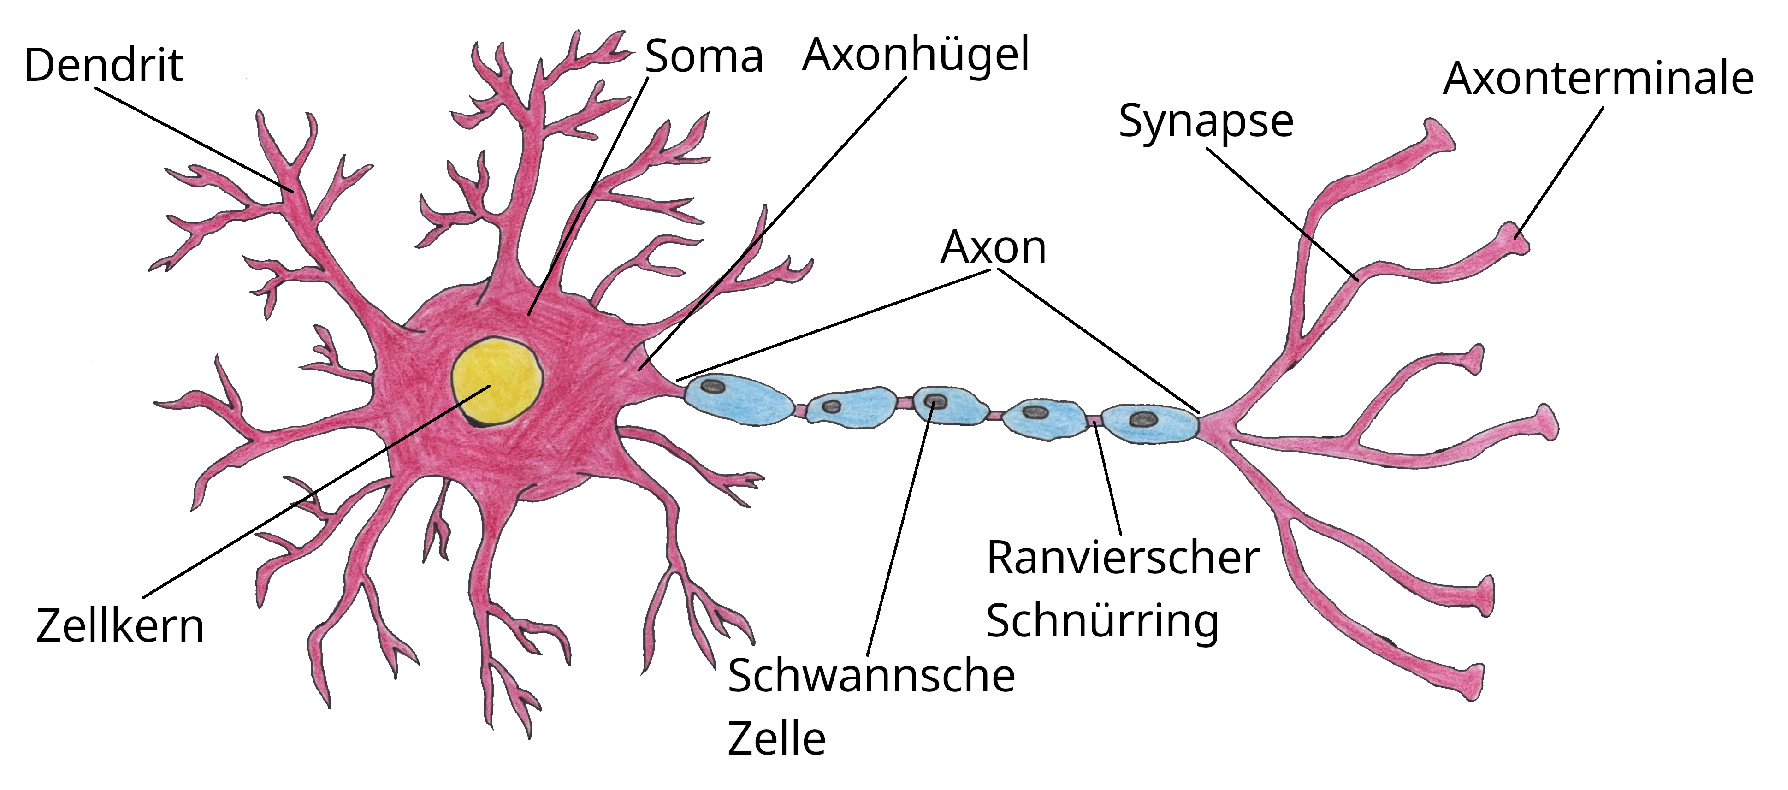
\includegraphics[width=0.8\textwidth]{content/chapter_basics/images/biological_neuron.eps}
	\centering
	\caption{Biologische Nervenzelle}
	\label{img:biological_neuron}
\end{figure}

Bei Nervenzellen werden elektrische Eingangssignale über Dendriten aufgenommen und in den Zellkern geleitet. Dort werden die eingehenden Signale zusammen geführt und es bildet sich das Aktionspotential. Übersteigt es das Schwellenpotential der Zelle, so wird das Signal über das Axon abgeleitet, die Nervenzelle \glqq \textit{feuert}\grqq.\vspace{0.2cm}

Die kleinste Einheit in künstlichen neuronalen Netzen sind die Neuronen. Sie sind den biologischen Nervenzellen nachempfunden.

\begin{figure}[!ht]
	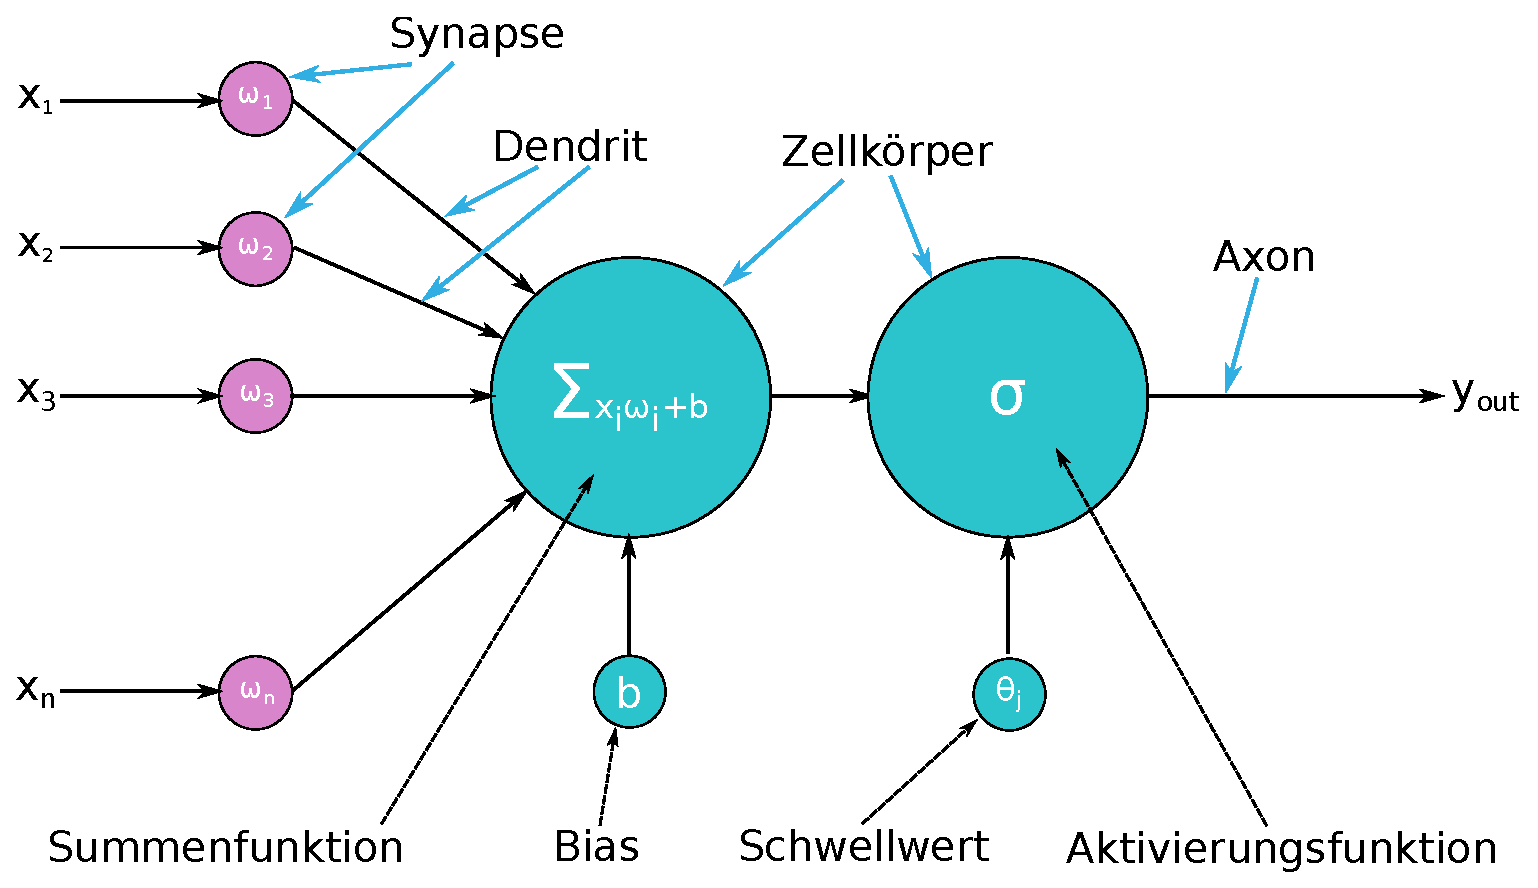
\includegraphics[width=0.8\textwidth]{content/chapter_basics/images/artificial_neuron.eps}
	\centering
	\caption{Künstliche Nervenzelle}
	\label{img:artificial_neuron}
\end{figure}

Sie haben als Eingangswert einen Vektor und als Ausgangssignal ein Skalar. Außer in der Eingabe Schicht ist jedes Eingangssignal $x_n$ ein Ausgangssignal $y_{out}$ eines anderen Neuron. Die Wichtungen der Eingangssignale modellieren den synaptischen Spalt zwischen zwei biologischen Nervenzellen. Dieser kann ebenfalls verstärkten oder hemmend wirken. Alle Eingangssignale zusammen mit den Wichtungen, werden durch die Summenfunktion aufaddiert. Im Anschluss wird das \gls{bias} mit eingerechnet. Die Formel \ref{eq:sum_function} zeigt die Summenfunktion für $n$ Eingangssignale mit Beachtung des Bias Wert.

\begin{equation} \label{eq:sum_function}
	y_{sum} = x_{1} + x_{2} + \dots + x_{n} + b
\end{equation}

Nach der Summenfunktion wird das Signal an die Aktivierungsfunktion übergeben. Diese Funktion leitet ein Signal erst weiter, wenn ein festgelegter Schwellwert überschritten wird. Die Analogie zur biologischen Nervenzelle ist das Aktionspotential, welches durch die Reize anderer Nervenzellen aufgebaut wird und wie beim künstlichen Neuron führt das Überschreiten eines Schwellenwertes dazu, dass das Neuron \glqq feuert\grqq. Die Formel \ref{eq:activation_function} zeigt das Verhalten einer \glqq Binary Step\grqq -Aktivierungsfunktion mit vorgegebenen Schwellenwert $S$.

\begin{equation}\label{eq:activation_function}
	\sigma (y_{sum}) = \left\{
	\begin{array}{cl}
		1: & y_{sum} > S \\
		0: & sonst \\
	\end{array}
	\right.
\end{equation}

Neben dieser einfachen Aktivierungsfunktion wie die \textit{Binary Step} gibt es viele weitere Aktivierungsfunktionen, beispielsweise die \textit{Sigmoidfunktion} oder \textit{ReLU (Rectified Linear Unit)} Funktion. Diese Aktivierungsfunktionen verwenden für die Berechnung immer das Ergebnis der Summenfunktion. Es gibt auch Aktivierungsfunktionen die alle Neuronen einer Schicht zur Berechnung verwenden. Zu diesen Funktionen zählen u.a. die Softmax- und die Maxout-Aktivierungsfunktion.\vspace{0.2cm}

Das eben beschriebene Neuronen-Modell ist ein einfaches Modell, welches oft in Netzen wie \textit{Feedforward Neural Netzwerke (FNN)}, \textit{Rekurrente neuronale Netze (RNNs)} oder \textit{Long Short-Term Memory Networks (LSTM)} Anwendung findet. Andere Neuronen-Modelle wie beispielsweise das \textit{Leaky-Integrate-And-Fire} Modell, finde seine Anwendung in gepulsten Netzwerken. Mit diesen mathematischen Modellen wird versucht das biologische Nervensystem nachzubilden, mit all seinen stärken und schwächen. Die Forschung hat in den letzten Jahren große Fortschritte gemacht, mit immer besser werdender Technik und Verständnis der biologischen ist das Potenzial der neuronalen Netze noch nicht erschöpft.


\subsection{Deep Learning}
Das Teilgebiet \textit{Deep Learning} versucht möglichst präzise Vorhersagen und Entscheidungen aus komplexen Daten zutreffen. Hierfür werden tiefe neuronale Netze verwendet. Das sind Netze mit vielen Hidden Layern zwischen der Ein- und Ausgabeschicht. Diese Strukturen erlauben die Verarbeitung und Analyse komplexer Datenmuster.


\section{Natural Language Processing}
Natural Language Processing ist ein Teilgebiet der Informatik und nutzt Deep Learning. NLP soll es digitalen Systemen in die Lage versetzen Texte und Sprachen zu erkennen, um diese zu verstehen und verarbeiten zu können. Dabei muss NLP die Bedeutung (Semantik) der Texte erkennen, die Grammatik und Beziehungen zwischen den Teilen der Sprache herstellen, Wortarten wie Verben, Adjektive und Nomen spezifizieren, sowie verschiedene Formen der Sprache beherrschen wie beispielsweise Prosa oder wissenschaftliches Schreiben.\vspace{0.2cm}

NLP wird aber auch in anderen Bereichen eingesetzt. Mithilfe von NLP können Bilder generiert, Suchmaschinen abgefragt, Chatbots für den Kundenservice betrieben werden und Sprachassistenten wie Amazon Alexa, MS Cortana und Apple Siri nutzen ebenfalls die NLP Techniken.\vspace{0.2cm}

Zunehmend findet NLP Einsatz im unternehmerischen Bereich. Hier werden vor allem Prozesse automatisiert um die Produktivität der Mitarbeiter zu steigern. Neben Aufgaben wie Kundensupport, Datenanalyse oder Dokumentenverwaltung kommt NLP auch in der Entwicklung von Software zum Einsatz. Hierbei werden fast alle Segmente der Entwicklung abgedeckt, von der Codegenerierung über Test und Qualitätsmanagement bis hin zur Bereitstellung.\vspace{0.2cm}

Die ersten große Erfolge hatte NLP mit neuronalen Netzen wie \textit{Feedforward Neural Networks} und \textit{Convolutional Neural Networks}, wie \cite{goldberg-2016} zeigt. Mit der Einführung von ChatGPT und BERT, wurde auch hier die neuen Transformer Modellen eingesetzt. Die Forschungen im Bereich NLP haben die großen Sprachmodelle erst ermöglicht.


\section{Large Language Model}
Die Teilgebiete Deep Learning und Natural Language Processing haben es den großen Sprachmodellen \acrshort{LLM} ermöglicht kommunikationsfähig zu werden. Sie verstehen Anfragen und können Antworten generieren. Die LLMs sind in der Lage Bilder und andere Medien wie Video oder Audio zu generieren.\vspace{0.2cm}

Die heutigen 

Diese Modelle wurden mit sehr großen Datenmengen trainiert und sind daher in der Lage natürliche Sprache zu verstehen.

\subsection{Grundlagen}
%Die großen Sprachmodelle oder Large Language Models sind darauf ausgelegt menschliche Sprache zu verstehen. Durch Textanalyse und Verarbeitung der Textbausteine durch \textit{Tokenisierung} und Vorhersage kommender Textbausteine.\vspace{0.2cm}

Die großen Sprachmodelle können menschliche Sprache arbeiten. Sie sind speziell für die Lösung  sprachbezogene Probleme geeignet, wie Textgenerierung, Klassifizierung und Übersetzung. Sie nehmen Anfragen sog. \textit{Prompts} entgegen und errechnen daraus die wahrscheinlichste Antwort. Des Weiteren können Prompts als Anweisung (instruction-tuning) oder in Dialogform (chat fine-tuning) gestellt werden. Die heutigen Sprachmodelle sind Modelle, welche die Transformer Technik verwenden.

Die grundlegende Funktionsweise der Large Language Models kann in vier Hauptkomponenten unterteilt werden,

\begin{enumerate}
	\item Tokenisierung: zerlegen der Texte in einzelne Token
	\item Embedding: Vergleiche mit anderen Vektoren und Einordnung in einer Gesamtstruktur
	\item Vorhersage: Wahrscheinlichkeit des nächsten Tokens berechnen
	\item Dekodierung: Auswahl der Ausgabestrategie
\end{enumerate}


\subsection{Grenzen und Probleme bei LLMs}
Auch wenn Künstliche Intelligenz mit ihren großen Sprachmodellen in vielen Bereichen der privaten Nutzer und in den Prozessen von Unternehmen immer präsenter wird, haben die diese auch Grenzen. Im folgen werden kurz die wichtigsten Grenzen und Probleme erläutert.

% https://www.unite.ai/de/Die-Bek%C3%A4mpfung-von-Halluzinationen-in-gro%C3%9Fen-Sprachmodellen-ist-ein-%C3%9Cberblick-%C3%BCber-modernste-Techniken/


\subsubsection{Ressourcenverbrauch}
Mit  dem Aufkommen der großen Sprachmodelle ist auch der Verbrauch an Ressourcen enorm angestiegen. Dabei stehen diese nur in einem begrenzten Maß zur Verfügung. Kleine und mittlere Unternehmen kommen hier schnell an ihre Grenzen und nutzen daher die Modelle der Anbieter wie OpenAI, Google oder Microsoft. Auch hier gilt Ressourcenbegrenzung, sodass die Modelle nicht unendlich groß werden können. Die folgenden Ressourcen, die hier genannt werden, haben direkten Einfluss auf die Modelle und deren Betrieb,

\begin{myitemize}
	\item Speicher
	\item Rechenleistung
	\item Netzwerk
	\item Energie
	\item Finanzen
\end{myitemize}

Im Lebenszyklus der großen Sprachmodelle werden Ressourcen in unterschiedlichen Mengen benötigen.\vspace{0.2cm}

%-------------------------------------------------------------------------------------------------


\subsection{Verständnis für die LLMs}
Viele Nutzer (Privatnutzer aber auch Firmen) wissen nicht, was hinter den großen Sprachmodellen steckt oder wie diese funktionieren. Diese Unwissenheit birgt die Gefahr, dass Nutzer nicht korrekte Eingabe in die LLMs übergibt und dann die Ergebnisse der LLMs falsch interpretieren oder die LLMs nicht korrekte Aussagen trifft. Werden aufgrund dieser falschen Ergebnisse Entscheidungen getroffen, können diese enorme finanzielle und personelle Einbußen nach sich ziehen. Zudem kann es weiterhin zu Desinformation, Diskriminierung, juristische Probleme und zum Vertrauensverlust in die Technologie führen.\vspace{0.2cm}

Um diesen Problemen bei Entwicklern entgegenzuwirken, sind vor, während und nach der Einführung einer LLM zur Codeentwicklung, die Nutzer aufzuklären. Sie müssen sich im klaren sein, dass LLMs Fehler produzieren und es erforderlich ist, die Ergebnisse zu validieren. Nur so kann die ein Vertrauensverlust und eine stetige Weiterentwicklung der Modelle erfolgen.

%-------------------------------------------------------------------------------------------------


\subsection{Auswahl der LLMs}
Die folgenden Modelle werden getestet und die Ergebnisse anschließend evaluiert.

\begin{table}[!ht]
	\begin{tabular}{|l|c|c|c|c|c|l|}
		\hline
		\textbf{Modell} & \textbf{Parameter} & \textbf{Größe} & \textbf{Sprache} & \textbf{offen} & \textbf{Ausführung}  & \textbf{Benchmark} \\
		\hline
		Qwen2.5-coder     & 32b &  19 GB & German & X & lokal  & HumenEval-XL \\
		%		CodeGeeX          &  9B & German &  & & lokal & HumenEval-XL \\
		Deepseek-coder-V2 & 16B & 8,9 GB & German &  X & lokal  & HumenEval-XL \\
		Llama3.1-Claude   &  8b & 4,7 GB & German &  X & lokal  & HumenEval-XL \\
		Llama3.2          &  3b & 2,0 GB & German &  X & lokal  & HumenEval-XL \\
		Codellama         & 13b & 7,4 GB & German &  X & lokal  & HumanEval-XL \\
		%		ChatGPT3.5        & & & German &  & online & HumenEval-XL \\
		Gemini Flash 1.5  & k.A.& k.A.   & German &  - & online & HumenEval-XL \\
		%		Opus              & & & German &  & online & HumenEval-XL \\
		%		Claude 3          & &  German & & & online & HumenEval-XL \\
		\hline
		\multicolumn{7}{|l|}{In Planung, wenn ich es schaffe} \\
		\hline
		Llama3.3          & 70b &  43 GB & German &  X & lokal  & HumanEval-XL \\
		\hline
	\end{tabular}
\end{table}

%-------------------------------------------------------------------------------------------------


\section{Koordinationsstrategien für LLMs}
Die Large Languarge Models haben große Leistungen auf dem Gebiet der Verarbeitung natürlicher Sprache gezeigt. Zunehmend arbeiten mehrere LLMs für diese Aufgaben zusammen. In diesem Fall spricht man von Agenten, die jeweils eine LLM darstellen können.\vspace{0.2cm}

Werden für unterschiedliche Aufgaben verschiedene Modelle verwendet, spricht man von Agenten. Ein Agent ist eine autonome Einheit. Sie ist in der Lage ihre Umwelt wahr zunehmen, Entscheidungen zu treffen und führt ihre Handlungen aus, um ein definiertes Ziel zu erreichen. Dies kann beispielsweise durch die \gls{bdi_architectur} umgesetzt werden. Jeder Agent ist auf unterschiedliche Aufgaben spezialisiert. In \cite{du-2024} werden Multi-Agenten-System mit Team aus der Softwareentwicklung verglichen und gleich gesetzt.\vspace{0.2cm}

Es gibt einige Methoden Large Language Model miteinander zu kombinieren, beispielsweise \glqq Pipeline-Architektur\grqq \ und \glqq Modular Approaches\grqq . Im Folgen Kapiteln werden die zwei Ansätze für die Zusammenarbeit von mehreren LLMs, \textit{Orchestrierung} und \textit{Multi-Agenten-System (MAS)} kurz erläutert.

\subsection{Orchestrierung von LLMs}
Bei der Orchestrierung von LLMs wird die Steuerung, der Agenten mittels eines zentralisierten Systems umgesetzt, es erfolgt eine koordinierte Nutzung. Meist wird ein Problem in Teilprobleme zerlegt und die Agenten bearbeiten Teilprobleme meist parallel. Die zentrale Steuerung entscheidet welche Teilaufgabe, welcher Agent am besten geeignet ist für die Lösung der Teilaufgabe.\vspace{0.2cm}

Die zentrale Rolle in der Orchestrierung von LLMs übernimmt dabei der Orchestrator. Dieser steuert die Aufgabenverteilung, koordiniert und kombiniert die Ergebnisse und leitet sie in die entsprechenden Agenten oder erstellt daraus die Antwort, außerdem kann er zusätzliche Aufgaben wie Fehlerbehandlung, Skalierung, Datenschutz und Sicherheit ausführen.\vspace{0.2cm}

Im Bereich der Softwareentwicklung mit Spezialisierung auf internetbasierte Anwendungen, bei der bestimmte Standards erwartet, spezielle Frameworks und Bibliotheken eingesetzt werden, könnte eine Orchestrierung bei der Umsetzung der Programmcodeerstellung wie folgt beschrieben, helfen. Bei der Lösung von Anforderungen sind nicht immer alle Agent beteiligt, vielmehr sucht der Orchestrator die jeweiligen optimalen Agenten aus.\vspace{0.2cm}

Der Orchestrator übernimmt auch hier die oben beschriebenen Aufgaben. Ein Frontend-Agent nutzt eines der großen Sprachmodelle, um Nutzeranforderungen in die Benutzeroberflächen der Anwendungen zu implementieren und könnte das Design verwalten. Gleichzeit wäre es möglich, dass dieser Agent Tools wie React.js oder Vue.js unterstützen. Für die serverseitigen Anwendungen ist der \textit{Backend-Agent} verantwortlich und verwaltet die Logik der Anwendung. Er könnte mit Frameworks wie Node.js, Express und Django umgehen. Um die Anwendung mit einer Datenbank auszustatten, kann ein \textit{Datenbank-Agent} eingesetzt werden. Er kennt verschiedenen Datenbanken wie MySQL oder PostgreSQL. Dieser verwaltet die Datenbank und deren Abfragen. Der \textit{Test-Agent} testet die Anforderung die von durch den Frontend-, Backenend- oder Datenbank-Agent umsetzt wurden.\vspace{0.2cm}

Ein letzter wichtiger Agent könnte noch der NLP-Agent sein. Dieser Agent nimmt natürliche Sprachanweisungen und Anforderungen entgegen, übersetzt diese in technische Anforderungen als Prompt für die Sprachmodelle. Die Ergebnisse der Bearbeitung werden zum Schluss von dem Agenten in eine vom Menschlichen verständliche Sprache überführt und zurückgegeben.

\subsection{Multi-Agenten-Systeme}
Multi-Agenten-Systeme (\acrshort{MAS}) bestehen ebenfalls aus mehreren Agenten. Im Gegensatz zur Orchestrierung sind Multi-Agenten-Systeme in ihrer Steuerung dezentralisiert. Alle Agenten haben unterschiedliche Lösungsansätze für ein Problem. Je nach deren Fähigkeit hat dieser auch seine ganz eigenen Ziele, welche zu den anderen Agenten entweder als \gls{collaborative} oder als \gls{competitive} ausgerichtet sind. Die Hauptarbeit zur Lösungsfindung eines Problems übernimmt der Agent, mit dem besten Lösungsansatz für das Problem. Die anderen Agenten können den ausführenden Agenten unterstützen. Um die beste Lösung zu finden, müssen die Agenten untereinander kommunizieren.  Teil der Kommunikation kann es sein, einfache Informationen austauschen, um eine gemeinsame Strategie fest zulegen oder um zu Verhandeln, welcher Agent die Lösung eines Problems übernimmt.\vspace{0.2cm}

Im Bereich der Webentwicklung mit MAS, könnte ein derartiges System wie folgt aussehen. Ein \textit{Frontend-Agent} ist für das Design und die Benutzeroberfläche verantwortlich. Hierbei erzeugt dieser Agent Ausgaben in HTML, JavaScript und CSS um die Oberflächen zu erstellen. Dazu kann er Frameworks, wie React verwenden und auf externe Designer Tool zugreifen. Ein weiterer Agent ist der \textit{Backend-Agent}, der für die serverseitige Anwendung zuständig ist. Er erstellt seine Funktionen in PHP, Python oder NodeJS. Der Backend-Agent hat Zugriff auf Frameworks und externe Bibliotheken. Der erstellt und verwaltet zudem die Datenbankoperationen (CRUD-Operations). Hinzu kommt noch ein \textit{Test-Agent}, welcher automatisierte Tests durchführt. Um die Funktionalität der Anwendung zu gewährleisten, arbeitet der Test-Agent mit dem Frontend- und Backend-Agent eng zusammen. Der Test-Agent stellt sicher, dass jegliche Codeänderung getestet wird und führt Unit-, Inetragtions- und End-to-End-Tests durch. Wird ein Fehler festgestellt, kann der Test-Agent ein Ticket erstellen oder direkt mit dem Frontend- oder Backend-Agenten kommunizieren.\vspace{0.2cm}

Ein weiterer Agent könnte ein \textit{Deploment-Agent} sein. Dieser führt automatische Depolyments in verschiedene Umgebungen (QA, Test oder Produktion) durch. Er ist in den Continuous Integration (CI) und Continuous Deployment (CD) Workflow integriert, welche die Bereitstellung auf verschiedenen Servern (VMware, Bare-Metal) und Cloud-Umgebungen (AWS, Azure, Google) bewerkstelligt. Des weitere könnten beispielsweise Security-Agent, Monitoring-Agent und Optimierungs-Agent Einsatz finden.\vspace{0.2cm}

Auch hier kann ein NLP-Agent zum Einsatz kommen und die Kommunikation zwischen Mensch und System managen.

% https://medium.com/scisharp/understand-the-llm-agent-orchestration-043ebfaead1f

%----------------------------------------------------------------

\section{Prompt Engineering}
Prompt Engineering optimiert die Antworten große Sprachmodelle, ohne Parameter, wie Bias und Gewichte des Models ändern zu müssen. Dieser Bereich hat in den letzten Jahren enorm an Bedeutung gewonnen und sich zu einer eigenen Disziplin im Bereich der Künstlichen Intelligenz entwickelt.\vspace{0.2cm}

Ein Prompt oder Anweisung muss entweder als Anweisung oder als Frage gestellt werden. Dies kann, wie in \cite{amatriain-2024} beschrieben, in Form von einer einfachen Anweisung bis hin zu detaillierten Beschreibungen oder spezifischen Aufgaben erfolgen.

\subsection{Prompt-Techniken}\label{subsec:prompt_technics}
Siehe Prompting Techniques Hinweise für die Optimierung von Prompts.
Die folgenden Techniken dienen dazu die Abfragen zu optimieren und somit eine bessere Antwort von den Sprachmodellen zu erhalten.

In dieser Arbeit werden hauptsächlich \textit{contextual augmentation} und \textit{Meta-Prompts} verwendet.\vspace{0.2cm}

\textbf{\textit{Kontextuelle Prompts}} haben neben der eigentlichen Eingabeaufforderung zusätzliche Informationen für die LLMs. Dazu gehören Kontextangaben, anzuwendende Programmiersprache, geforderte Bibliotheken, Angaben der Zielgruppe und Definition über die auszugebende Struktur wie Methoden oder Klassen.\vspace{0.2cm}

Beispiel für einen kontextuellen Prompt:

\textit{Du bist ein Erfahrener PHP Programmierer, hier deine Aufgabe. Erstelle eine PHP-Funktion, die eine Liste von Ganzzahlen sortiert und zugibt.}\vspace{0.2cm}

Ausgabe der LLM:

\begin{lstlisting}[language=PHP]
	function sortiere_und_gebe_aus($zahlen) {
		// Die Liste wird nach aufsteigender Reihenfolge sortiert
		sort($zahlen);
		
		// Die sortierte Liste wird ausgegeben
		foreach ($zahlen as $zahl) {
			echo $zahl . " ";
		}
	}
\end{lstlisting}

Diese Art der Prompts können hilfreich sein, wenn Erweiterungen oder Änderungen in bestehende Programme erfolgen. Hier sind oft schon Standards oder Bibliotheken definiert.\vspace{0.2cm}

\textbf{\textit{Meta-Prompts}} sind Prompts, die eine LLMs anweisen, einen Prompt zu erstellen.\vspace{0.2cm}

Meta-Prompt Beispiel:

\textit{Du bist eine Prompt-Engineer und hier ist deine Aufgabe. Schreibe einen Prompt, der eine PHP-Funktion generiert, die eine Methode erstellt, die eine Liste von Ganzzahlen sortiert.}\vspace{0.2cm}

Ausgabe der LLM:

\textit{Schreibe eine PHP-Funktion namens} \texttt{sortiereZahlen}\textit{, die ein Array von Ganzzahlen als Parameter entgegennimmt. Die Funktion soll das Array in absteigender Reihenfolge sortieren und das sortierte Array zurückgeben. Nutze eine geeignete PHP-Funktion für die Sortierung.}\vspace{0.2cm}

Es gibt weitere Prompt-Typen, die nicht relevant für diese Arbeit sind. Eine Zusammenfassung von Methodiken und deren Beurteilung kann \cite{chen-2023} entnommen werden.


\subsection{Grenzen beim Prompt-Engineering für LLMs}
Trotz der bemerkenswerten linguistischen Leistung, stoßen große Sprachmodelle an ihre Grenzen, unter anderem wie in \cite{amatriain-2024} beschrieben,

%\section{Relevante Arbeiten}
%In \cite{zhou-2022} wird der Prompt-Optimierungsprozess als Black-Box interpretiert. Der mit minimalen Eingaben ein menschenähnliches Niveau erreichen soll.


\subsubsection{Prompttemplates}
Um die Eingaben für Programmierer oder Nutzer und dessen Anfragen an LLMs zu vereinfachen, können Propmt-Templates verwendet werden. Diese eigenen sich im besonderen Maße für automatisierte Prompts.

\begin{lstlisting}[language=text]
	Erstelle eine [Programmiersprache] Funktion namens [Funktionsname], die 
	[Beschreibung der Funktion]
	. Die Funktion soll folgende Parameter verwenden:
	[Liste der Parameter]
	. Die Funktion soll folgende Bedingungen erfüllen:
	[Liste der Bedingungen: z.B. Fehlerbehandlung, bestimmte Algorithmen]
	. Die Ausgabe der Funktion soll in folgendem Format sein:
	[Erwartetes Ausgabeformat]
\end{lstlisting}

%-------------------------------------------------------------------------------------------------


%\section{Grundlagen bei der Entwicklung von Webanwendungen}
%Webanwendung

\section{Grundlagen der Webentwicklung}
In diesem Unterkapitel soll kurz auf Anforderungen der Webentwicklung eingegangen werden.


\subsection{Programmiersprachen}
Grundsätzlich kann jede Programmiersprache verwendet werden. Es gibt jedoch Programmiersprachen, die explizit für Webanwendungen entwickelt wurden und einige Funktionen mitbringen, welche die Entwicklung vereinfachen. Die meisten visuellen Anwendungen erstellen HTML (\textbf{H}yper\textbf{T}ext \textbf{M}arkup \textbf{L}anguage) Code als Grundgerüst und generieren CSS (\textbf{C}ascading \textbf{S}tyle \textbf{S}heets) Dateien für das Layout, die als Standardformatierungssprache gilt. Anwendungen die als RestAPI (\textbf{A}pplication \textbf{P}rogramming \textbf{I}nterface) fungieren liefern meist Ausgaben in Form von JSON (\textbf{J}ava\textbf{S}cript \textbf{O}bject \textbf{N}otation) aus. Neben JSON Format gibt es weitere beispielsweise XML () oder YAML (\textbf{Y}AML \textbf{A}in’t \textbf{M}arkup \textbf{L}anguage).\vspace{0.2cm}


\subsection{Entwicklung}
Bei der Entwicklung von Webseiten werden längst schon die selben Prozesse und Tools verwendet wie bei anderen Softwareprojekten. Auch hier finden Tolls wie GitLab\footnote{\href{https://about.gitlab.com/}{Gitlab} ist eine webbasierte Anwendung die Issue-Traking, CI/CD Pipelines, Dokumentation und mehr für Entwickler anbietet.} und Jenkins\footnote{\href{https://www.jenkins.io/}{Jenkins} ist ein webbasiertes Tool für die kontinuierliche Integration welches viele Build-Tools, wie Ant und Maven integriert, Testtols wie JUnit und Emma bietet, sowie Verwaltungssystem wie CVS, Subversion und Git unterstützt. Jenkins kann durch viele Plugins erweitert werden.} Anwendung. Gerade in der Entwicklung von cloudbasierten Anwendungen kommen Containertools wie Docker\footnote{Durch die Containerisierung mit \href{https://www.docker.com/}{Docker} können Anwendungen und deren Umgebungen einfach bereitgestellt und bei bedarf skaliert werden. Docker bietet eine Vielzahl von einsatzbereiten Container an, die einzeln oder in Clustern laufen können.} in Verbindung mit Kubernetes\footnote{\href{https://kubernetes.io/}{Kubernetes} ist  Orchestrierungstool für Dockercontainer das von Google entwickelt wurde. Neben den Container-Anwendungen verwaltet Kubernetes auch die Umgebung für Container, wie beispielsweise Netzwerke.} zum Einsatz. Diese Tools lassen sich hervorragend in CI/CD Pipelines integrieren. An deren Anfang steht auch hier der Entwickler, welcher durch KI Unterstützung erhalten kann.


\subsubsection{Einsatz von KI}
Der Einsatz von Künstlicher Intelligenz kann in allen Entwicklungsphasen eingesetzt werden, angefangen von der Codegenerierung über die Bereitstellung mittels Pipeline bis zur Inhaltserstellung.\vspace{0.2cm}

Der Einsatz von NL2Code steck hier noch in den Anfängen, bietet aber sehr gute Ansätze viele Aufgaben zu automatisieren oder als Werkzeug um die Entwicklung effizienter zu gestalten.\vspace{0.2cm}

Die Codegenerierung für Designelemente kann ebenso mittels NL2Code erfolgen wie komplexe Backendfunktionalitäten. Ebenso kann die vorherige Konzeption durch eine LLM erfolgen.

%-------------------------------------------------------------------------------------------------


\section{Benchmark für LLM}
Bei der Evaluierung großer Sprachmodell hinsichtlich des generierten Codes, gibt es einige Herausforderungen. Herkömmliche Methoden, wie BLUE-Score misst die Textähnlichkeiten nicht aber die funktionale Korrektheit des Codes und vernachlässigt auch den Kontext, in dem der Code erstellt wurde. Ein generierter Code kann in seiner Lösung stark von einer vorgegebenen Beispiellösung abweichen, trotzdem aber seine Funktionalität erfüllen. Menschliche Programmierer würden das mit verschiedenen Unit-Tests überprüfen, aus diesem Grund sollte der Code mit einer weiteren Methode geprüft werden.\vspace{0.2cm}

Als Benchmark für die Bewertung der großen Sprachmodelle wird der HumanEval-XL verwendet, welche unter \href{https://github.com/FloatAI/humaneval-xl/tree/main}{https://github.com/FloatAI/humaneval-xl/tree/main} heruntergeladen werden können.\vspace{0.2cm}

Der Benchmark besteht aus Prompt, die wie folgt aufgebaut sind,

\begin{myitemize}
	\item \textbf{task\_id}: Kennung der Datenprobe
	\item \textbf{prompt}: Anfrage für das Modell, Funktionsheader und Docstring
	\item \textbf{entry\_point}: Einstiegspunkt für den Test
	\item \textbf{test}: Test für die geforderte Funktion
	\item \textbf{description}: Beschreibung der Aufgabe
	\item \textbf{language}: Kennung der Programmiersprache
	\item \textbf{canonical\_solution}: Lösung für das Problem
	\item \textbf{natural\_language}: Ländersprache in der Datei
\end{myitemize}

Durch diesen Aufbau werden neben dem eigentlichen Prompt ein Test, eine vorgeschlagene Lösung mitgeliefert, sowie weitere Metadaten mit geliefert. Die Abbildung \ref{img:code_generation_humaneval} zeigt den Aufbau und damit alle wichtigen Bereiche des Benchmark-Tests.

\begin{figure}[!ht]
	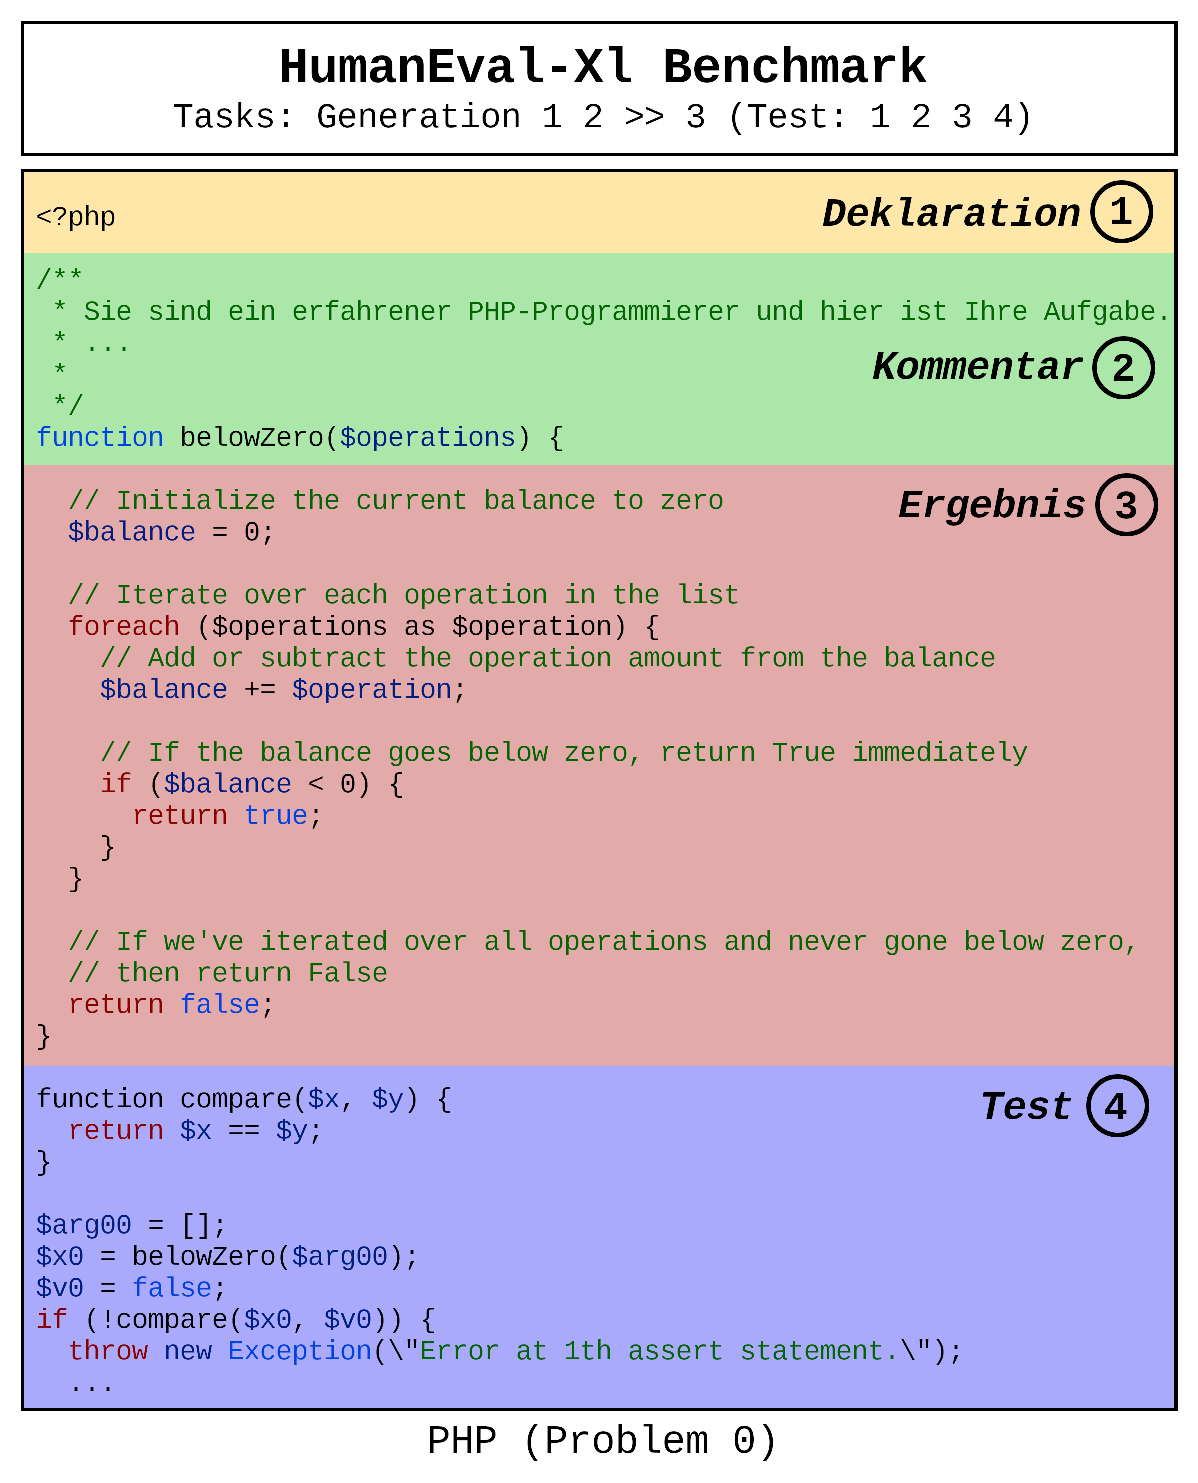
\includegraphics[width=0.8\textwidth]{content/chapter_intruduction/images/code_generation_humaneval_x.eps}
	\centering
	\caption{Codegeneration}
	\label{img:code_generation_humaneval}
\end{figure}

%-------------------------------------------------------------------------------------------------
